Differential calculus is all about finding the slope of a curve. 
First, let's consider a normal case, finding the slope of a straight line. 
We take in two points, and find the change in x and change in y ($\Delta x$ and $\Delta y$). 
This can be written as $\frac{\Delta y}{\Delta x}$ or $\frac{\text{rise}}{\text{run}}$.

\begin{figure}[H]
\caption{Average Slope}
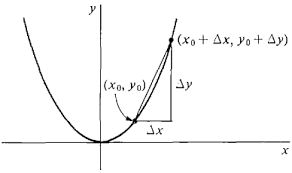
\includegraphics[scale=1]{../download.png}
\end{figure}

The above diagram illustrates this process on a curve. 
We pick two points on the line and find the average slope. 
However, this process is clearly not very accurate. 
Imagine that we move the two points closer and closer together. 
The closer they are, the more accurate the slope is for that small section of line, until eventually we make it so that there is only one point. 
That is, we are finding instantaneous slope, or the slope at one point of the line.

The derivative does that for the whole line, taking in a function and giving a new function that represents the slope. 
For example, let's say we shoot a cannonball.

\begin{figure}[H]
\caption{Trajectory of cannonball}
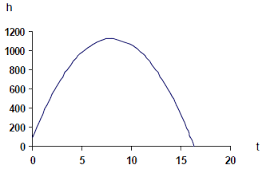
\includegraphics[scale=1]{../imgres.png}
\end{figure}

Here, the y-axis represents the height of the cannonball in meters and the x-axis indicates time in seconds. 
Notice that at the beginning the slope is positive, until eventually the graph reaches its peak and the slope is zero, and then the graph starts going down and the slope becomes negative. 
The derivative of this graph would then look something like this:

\begin{figure}[H]
\caption{Derivative of trajectory of cannonball}
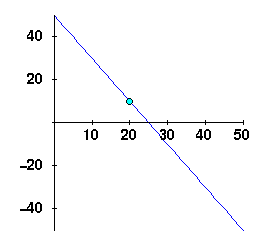
\includegraphics[scale=0.8]{../derivative.png}
\end{figure}

This is what is happening "behind the scenes" when we calculate derivatives.
However, it is important to note that, going back to the example of the cannonball, where the cannonball started does not affect the slope. 
If the whole graph is shifted up or down, the slope stays the same (as long as the proportions are kept the same). 
This, it turns out, is why we need to add the $c$ in a indefinite integral. 

Derivatives and integrals are inverses of each other. 
That is, they undo each other, like division undoes multiplication and subtraction undoes addition. 
So, because when going from an integral back to a derivative there is some uncertainty which graph you are looking at (parallel lines, for instance, have the same slope, but they have different "heights"), you have to add the $c$ when solving an indefinite integral.

Below is a table with some solutions to various derivatives. Note that $c$ is a constant and $n$ is non-zero. Note that the $'$ symbol is pronounced prime, and is another way to write that we are taking the derivative. 


\begin{tabular}{c|c}
    $f(x)$ & $\frac{df}{dx} = f'$\\
    \hline
       $7$  & $0$ \\
        $c$ & $0$ \\
        $x$ & $1$ \\
        $cx$ & $c$ \\
        $x^2$ & $2x$ \\
        $cx^2$ & $2cx$ \\
        $x^3$ & $3x^2$ \\
        $x^n$ & $nx^{n-1}$ \\
        $\sin x$ & $\cos x$ \\
        $\cos x$ & $-\sin x$ \\
        $- \sin x$ & $- \cos x$ \\
        $-\cos x$ & $\sin x$
\end{tabular}

Like integrals, derivatives are distributive over addition.
There are some interesting rules that make working with derivatives easier: the product rule, the quotient rule, and the chain rule. 

Let's start with the chain rule. 
If we have a function within a function in a derivative, like $\sin(\cos(x))$, we can assign a name to each function, like $g(x) = \cos(x)$ and $h(x) = \sin(x)$, and then follow this simple rule: $h'(g(x)) \cdot g'(x)$. 
So what does this mean? 
Well, let's plug it in. 
Plugging this in gives $\sin'(\cos(x)) \cdot \cos'(x)$. 
So the derivative of $\sin$ is $\cos$, so we write $\cos(\cos(x))$ for the first part, and the derivative of $\cos$ is $-\sin$, so we write $-\sin(x)$ for the second part. 
So now we have $\cos(\cos(x)) \cdot -\sin(x)$. 
This is the derivative of our original function.

Now, let's examine the product rule. 
If we have two functions, $u(x)$ and $v(x)$, and we want to take the derivative of $u\cdot v$, then we can do $u \cdot \frac{dv}{dx}+ v\cdot\frac{du}{dx}$. 
In other words, we multiply the first function by the derivative of the second function and then add the second function times the derivative of the first. 
For example, if we have $\sin(x)\cdot\cos(x)$ we would do $u(x) = \sin(x)$ and $v(x) = \cos(x)$. 
Then we would plug it in to our formula: $\sin(x)\cdot\frac{d}{dx}\cos(x) + \cos(x)\cdot\frac{d}{dx}\sin(x)$ which simplifies to $\sin\cdot -\sin(x) + \cos(x)\cdot\cos(x)$ or $-\sin^2(x)+\cos^2(x)$, which is our derivative of the original function.

Finally, the quotient rule. 
If we have two functions, $g(x)$ and $h(x)$, and we wish to take the derivative of $\frac{g(x)}{h(x)}$, we can follow the rule $\frac{g'(x)h(x)-h'(x)g(x)}{[h(x)]^2}$. 
While this may look rather complicated, it really isn't too bad. 
Let's use the example of $g(x) = \sin(x)$ and $h(x) = \cos(x)$. 
We plug it all in to get $\frac{\sin'(x)\cdot\cos(x) -\cos'(x)\cdot\sin(x)}{\cos^2(x)}$
which simplifies to $\frac{\cos(x)\cdot\cos(x)--\sin(x)\cdot\sin(x)}{\cos^2(x)} = \frac{\cos^2(x)+sin^2(x)}{\cos^2(x)} = \sin^2(x)$. 
So therefore, $\sin^2(x)$ is our derivative.

Now, let's say you forget this rule, or come across something you can't use these rules on. In this case, you can use the formal definition of a derivative. When looking at this definition, remember that $\Delta$ means "change in" whatever variable comes afterwards (i.e., $\Delta x$ means the change in x). Given a function $f(t)$, the derivative of $f(t)$ ($\frac{df(t)}{dt}$) is \begin{equation}
    \lim\limits_{\Delta t\rightarrow 0}\frac{\Delta f}{\Delta t} = \lim\limits_{\Delta t\rightarrow 0}\frac{f(t+\Delta t)-f(t)}{\Delta t}
\end{equation}
Let's try using this on a derivative - say, the derivative of $f(t)$ where $f(t) = t^2$. We have to solve $\lim\limits_{\Delta t\rightarrow 0}\frac{f(t+\Delta t)-f(t)}{\Delta t}$. Remember that the rule is that the input to $f$ must be squared, so for the first term, we need to square $t+\Delta t$ - $(t+\Delta t)(t+\Delta t) = t^2+t\Delta t+t\Delta t + \Delta t^2 = t^2+2t\Delta t+\Delta t^2$. That's the first term on top of the fraction. The second term is just $f(t)$ - which we've been told equals $t^2$. Since we subtract this from the first term, the two cancel, leaving $\frac{2t\Delta t+\Delta t^2}{\Delta t}$. We then divide, getting $2t+\Delta t$. Now we have to apply the limit in front. Remember that if there will be no mathematically impossible results, we can just plug in the limit - i.e., in this case, $2t+0$ or just $2t$, which is our result. We can of course check this using our earlier exponent rule (which we can actually derive; see exercise six and solution), and $2t$ is still the result.
